\part{Marc Pràctic}

\chapter{Redacció d'aquest treball amb \LaTeX}

Tot aquest treball escrit està redactat en LaTeX, que és un sistema de composició textos orientat a la creació de documents profesional, especialment s'utilitza en la redacció d'articles científics.
LaTeX no és un sistema WYSIWYG, que significa "Allò Que Veus És Allò Que Obtens". En lloc d'això, amb LaTeX, treballes amb un text sense format amb etiquetes. Aquestes etiquetes són instruccions del que ha de ser el text.
Un exemple amb seccions i subseccions a LaTeX es veuria com al listing \ref{lst:prova-latex} i la figura \ref{fig:prova-latex}.

\begin{lstlisting}[style=latex, caption={Exemple de Secció i Subsecció a LaTeX}, label={lst:prova-latex}]
\section{Secció de Prova}
Text de prova.

\subsection{Subsecció de prova}

\end{lstlisting}

\begin{figure}[h]
    \centering
    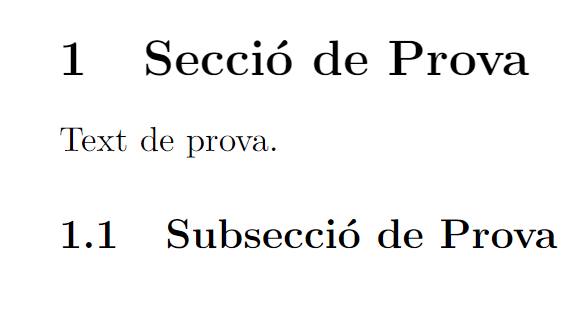
\includegraphics[width=0.5\textwidth]{img/figures/prova-codi-latex.png}
    \caption{Exemple de Secció i Subsecció a LaTeX}
    \label{fig:prova-latex}
\end{figure}


A més a més, he estat mantenint un control de versions a Github que es pot veure a \href{https://github.com/PolSances13/TDR}{PolSances13/TDR}

\section{Les Figures del Document}

Les figures del document són totes d'elaboració pròpia, tant les imatges com els cubs representats al document. 
Els cubs estan fets també a LaTeX, utlitzen el paquet TikZ, i dins d'aquest paquet es troben els de rubikcube i rubikrotation per fer els cubs i que es mostrin amb els moviments inserits.
El codi per formar un cub es pot veure al listing \ref{lst:prova-cub} i el resultat a la figura \ref{fig:cubs-latex}, hi ha moltes etiquetes, però el que mana a l'hora de "fer els moviments" al cub i que es mostri en una orientació o altra són les etiquetes de "RubikRotation" i "DrawRubikCube". 


\begin{lstlisting}[style=latex, caption={Exemple de Cubs fets amb el paquet rubikcube}, label={lst:prova-cub}]
    \begin{figure}[htbp]
        \centering
        \begin{subfigure}
            \centering\RubikCubeSolvedWY
            \RubikRotation{Y,M2,S2,E2}
            \ShowCube{7cm}{0.5}{\DrawRubikCubeLU}
        \end{subfigure}
        \begin{subfigure}
            \centering\RubikCubeSolvedWY
            \RubikRotation{M2,S2,E2}
            \ShowCube{7cm}{0.5}{\DrawRubikCubeRD}
        \end{subfigure}
    \end{figure}
\end{lstlisting}

\begin{figure}[htbp]
    \centering
    \begin{subfigure}
        \centering\RubikCubeSolvedWY
        \RubikRotation{Y,M2,S2,E2}
        \ShowCube{7cm}{0.5}{\DrawRubikCubeLU}
    \end{subfigure}
    \begin{subfigure}
        \centering\RubikCubeSolvedWY
        \RubikRotation{M2,S2,E2}
        \ShowCube{7cm}{0.5}{\DrawRubikCubeRD}
    \end{subfigure}
    \caption{Cubs de demostració fets amb el paquet rubikcube}
    \label{fig:cubs-latex}
\end{figure}


Els trossos de codi que es mostren durant l'explicació de l'App al capítol \ref{cha:python} són elaborats amb el paquet listings i s'escriu de la següent manera el codi \ref{lst:prova-hello}

\begin{lstlisting}[style=latex, caption={Exemple de codi Hello world mostrat amb el paquet listings}, label={lst:prova-hello}]
    \begin{lstlisting}[language=Python, style=colorEX, caption=Inici de la classe i especificació de la finestra]
        print("Hello World")
     \end{lstlisting }
\end{lstlisting}

El meu tutor em va recomanar fer-ho en LaTeX i ell m'ha guiat durant tot el treball, també he buscat el funcionament d'algunes pel meu compte. \cite{learnlatex2023} \cite{RubiksCubeTikz} \cite{HeaderambFancy}  
